\documentclass[../../D1.tex]{subfiles}

\begin{document}
Neural network compression is necessary due to storage related issues that often arise on resource contrained systems due to the high number of parameters that modern DNNs tend to use, state-of-the-art CNNs can have upwards of hundreds of millions of parameters. 
Different compression methods can result in variuous underlaying representations of the weight matrices, particularly with respect to its sparsity. 
Compression techniques that preserve the density of the weight matrix tend to result in inference acceleration on general-purpose processors\autocite{lebedevSpeedingupConvolutionalNeural2015,zhangAcceleratingVeryDeep2016}, not all techniques preserve this density and can result in weight matrices with various degrees of sparsity which in turn have varing degrees of regularity. 
These techniques, the resulting representations of parameters, and their consequences will be discussed in this section.

\subsubsection{Pruning}\label{sec:Pruning}
Network pruning is the process of removing unimportant connections, leaving only the most informative connections.
Typically pruning is performed by iterating over the following 3 steps: begin by evaluating the importance of parameters, next the least important parameters are pruned, and finally some fine tuning must be performed to recover accuracy.
There has been a substantial amount of research into how pruning can be used to reduce overfitting and network complexity~\autocite{hansonComparingBiasesMinimal,hassibiSecondOrderDerivatives,lecunOptimalBrainDamage,stromPhonemeProbabilityEstimation1997}, but more recent research shows that some pruning methodologies can produce pruned networks with no loss of accuracy~\autocite{hanLearningBothWeights2015}.

\begin{figure}[H]
    \begin{center}
        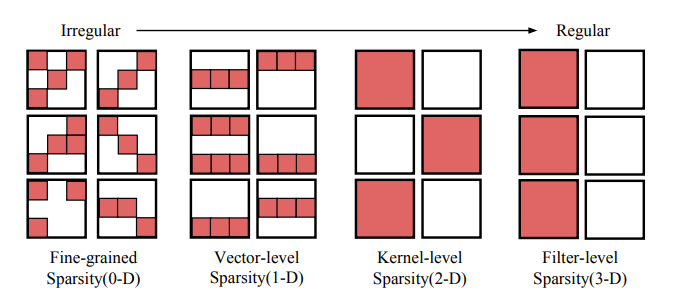
\includegraphics[width=0.7\textwidth]{sparsity_structure.png} 
    \end{center}
    
    \caption{Sparse structures in a 4-dimensional weight tensor. Regular sparsity makes hardware acceleration easier.\\ \textbf{(Adopted figure from~\autocite{maoExploringRegularitySparse2017})}}
    \label{fig:SparsityRegularity}   
\end{figure}

This process of pruning the weight matrix within a DNN results in a sparse matrix representation of weights, where the degree of sparsity is determined by the pruning algorithm being used and hyperparameters that can be tuned for the situation, such as how much accuracy loss is considered acceptable, and to what degree the neural network needs to be compressed. 
The pattern of sparsity in a weight matrix is a fundamental factor when considering how to accelerate a pruned neural network~\autocite{maoExploringRegularitySparse2017}, this is known as the \textbf{granularity of sparsity}.
Figure~\ref{fig:SparsityRegularity} provides a visual representation of granularity of sparsity, the spectrum of granularity usually falls between either \textbf{fine-grained (unstructured)} or \textbf{course-grained (structured)}, pruning techniques are also categorised by the aformentioned granularities.


The influential paper Optimal Brain Damage by LeCun et al~\autocite{lecunOptimalBrainDamage} was the first to propose a very fine-grained pruning technique by identifying and zeroing individual weights within a network.
Fine-grained pruning results in a network that can be challenging to accelerate without custom hardware such as proposed in~\autocite{hanEIEEfficientInference2016,parasharSCNNAcceleratorCompressedsparse2017}, a software solution has been theorized by Han et al~\autocite{hanDeepCompressionCompressing2016} that would involve developing a customized GPU kernel that supports indirect matrix entry lookup and a relative matrix indexing format, see Section~\ref{sec:Quantisation} for further details on the necessary steps for this technique.


Coarse-grained pruning techniques such as channel and filter pruning preserve the density of the network by altering the dimensionality of the input/output vectors, channel pruning involves removing an entire channel in a feature map, filter level pruning likewise removes an entire convolutional filter. 

This style of pruning however can have a significant impact on the accuracy of the network, but as demonstrated by Wen et al~\autocite{wenLearningStructuredSparsity2016}~accelerating networks with very course-grained pruning is straightforward because the model smaller but still dense, so libraries such as~\acrshort{blas} are able to take full advantage of the structure. 




\subsubsection{Quantisation}\label{sec:Quantisation}
%Define Quantisation
Most off-the-shelf DNNs utilise floating-point-quantisation for their parameters, providing arbitrary precision, the cost of this precision can be quite high in terms of arithmetic operation latency, high resource use and higher power consumption.
However this arbitrary precision is often unnecesssary, extensive research~\autocite{jacobQuantizationTrainingNeural2018,maOptimizingLoopOperation2017} has shown reducing the precision of parameters can have an extremely small impact on the accuracy.
Quantisation can be broadly categorised into two groups: non-linear quantisation and fixed-point (linear) quantisation. 


\textbf{Fixed-point quantisation} is the process of limiting the floating point precision of each parameter (and potentially each activation) within a network to a fixed point. 

In the extreme fixed-point quantisation can represent each parameter with only 1 bit (also known as binary quantisation) with up to a theoretical 32x compression rate (in practice this is often closer to 10.3x)~\autocite{chenDeepLearningMobile2020}, Umuroglu et al.~\autocite{umurogluFINNFrameworkFast2017} used binary quantisation with an \acrshort{fpga} and achieved startling classification latencies (0.31$\mu$s on the MINIST dataset) while maintaining 95.8\% accuracy, this is largely because the entire model can be stored in on-chip memory this is discussed further in Section~\ref{sec:MemAlloc}.

\begin{figure}[H]
    \begin{center}
        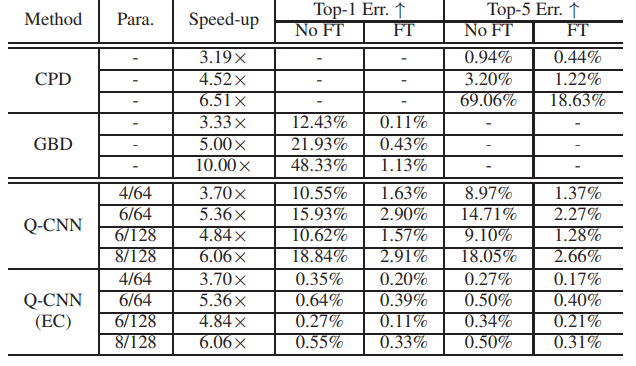
\includegraphics[width=1\textwidth]{QuantisationSpeedup.png} 
    \end{center}
    
    \caption{Comparison of the speed-up when quantising a convolutional layer in Alexnet, 3 different methods.\\ \textbf{(Adopted figure from~\autocite{wuQuantizedConvolutionalNeural2016})}}
    \label{fig:QuantisationSpeedup}   
\end{figure}

\textbf{Non-linear Quantisation} is a technique where the weights are split into groups and then assigned a single weight, this grouping can be accomplished in a number of ways, Gong et al.~\autocite{gongCompressingDeepConvolutional2014} used vector quantisation with $k$-means clustering and achieved compression rates of up to 24x while keeping the difference of top-five accuracy within 1\%. Wu et al.~\autocite{wuQuantizedConvolutionalNeural2016} quantised both FC and convolutional layers in Alexnet using their Q-CNN framework



The paper Deep Compression by Han et al~\autocite{hanDeepCompressionCompressing2016} quantisation and weight sharing is taken a step further.
First the weights are pruned and quantized, next clustering is employed to gather the quantized weights into bins (whose value is denoted by the centroid of that bin) finally an index is assigned to each weight that points to the weights corresponding bin, the bins value is the centroid of that cluster, which is further fine-tuned by subtracting the sum of the gradients for each weight in the bin their respective centroid see Fig.~\ref{fig:QuantisationClust}.  

\begin{figure}[H]
    \begin{center}
        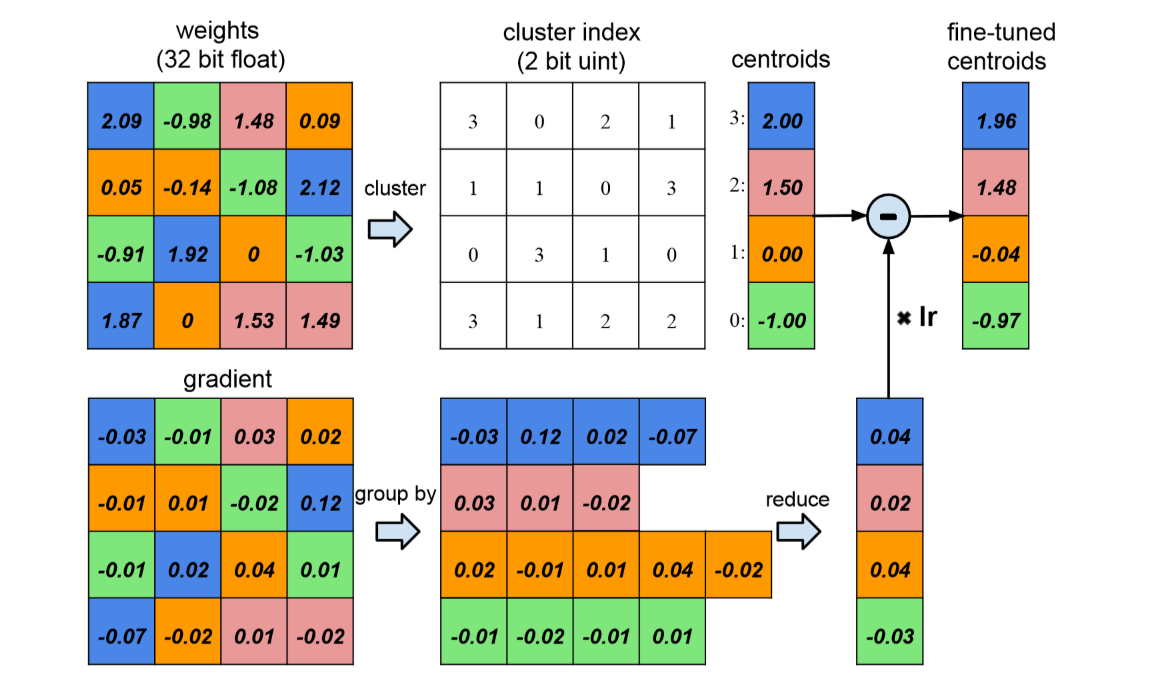
\includegraphics[width=1\textwidth]{quantization_clustering.png} 
    \end{center}
    
    \caption{Weight sharing by quantisation with centroid fine-tuning using gradients\\ \textbf{(Adopted figure from~\autocite{hanDeepCompressionCompressing2016})}}
    \label{fig:QuantisationClust}   
\end{figure}


\end{document}
